\documentclass[tikz,border=8pt]{standalone}
% Shared TikZ style for synorg platform diagrams. Each diagram \input's this
% inside a standalone document. Palette tracks the Material "teal" site theme so
% figures read as one system in light mode (SVGs are theme-neutral otherwise).
\usetikzlibrary{arrows.meta,positioning,shapes.geometric,fit,backgrounds,calc,decorations.pathreplacing}

\definecolor{synteal}{HTML}{00897B}   % primary
\definecolor{synfill}{HTML}{E0F2F1}   % light fill
\definecolor{synamber}{HTML}{B26A00}  % warning / lend
\definecolor{synred}{HTML}{B00020}    % deny / danger
\definecolor{syngrey}{HTML}{5F6368}   % muted

\tikzset{
  >=Stealth,
  font=\sffamily\small,
  box/.style={draw=synteal,line width=0.6pt,rounded corners=2pt,fill=synfill,
              inner sep=5pt,align=center},
  plane/.style={draw=synteal,line width=0.8pt,rounded corners=3pt,fill=synfill,
                inner sep=8pt,align=center},
  state/.style={draw=synteal,line width=0.7pt,circle,fill=synfill,inner sep=3pt,
                minimum size=11mm,align=center,font=\sffamily\footnotesize},
  decision/.style={draw=synteal,line width=0.7pt,diamond,aspect=2,fill=synfill,
                   inner sep=1pt,align=center,font=\sffamily\footnotesize},
  deny/.style={draw=synred,fill=synred!8,text=synred},
  warn/.style={draw=synamber,fill=synamber!10},
  flow/.style={->,line width=0.6pt,draw=syngrey},
  flowlbl/.style={font=\sffamily\footnotesize,text=syngrey,inner sep=2pt},
  note/.style={font=\sffamily\footnotesize\itshape,text=syngrey},
}

\begin{document}
% Verify-before-terminate carve loop (capacity-carve.md). The reservation, not
% the instance, is the thing protected: every failed hold aborts the step and
% NEVER releases capacity. All three verify gates fail closed to one ABORT.
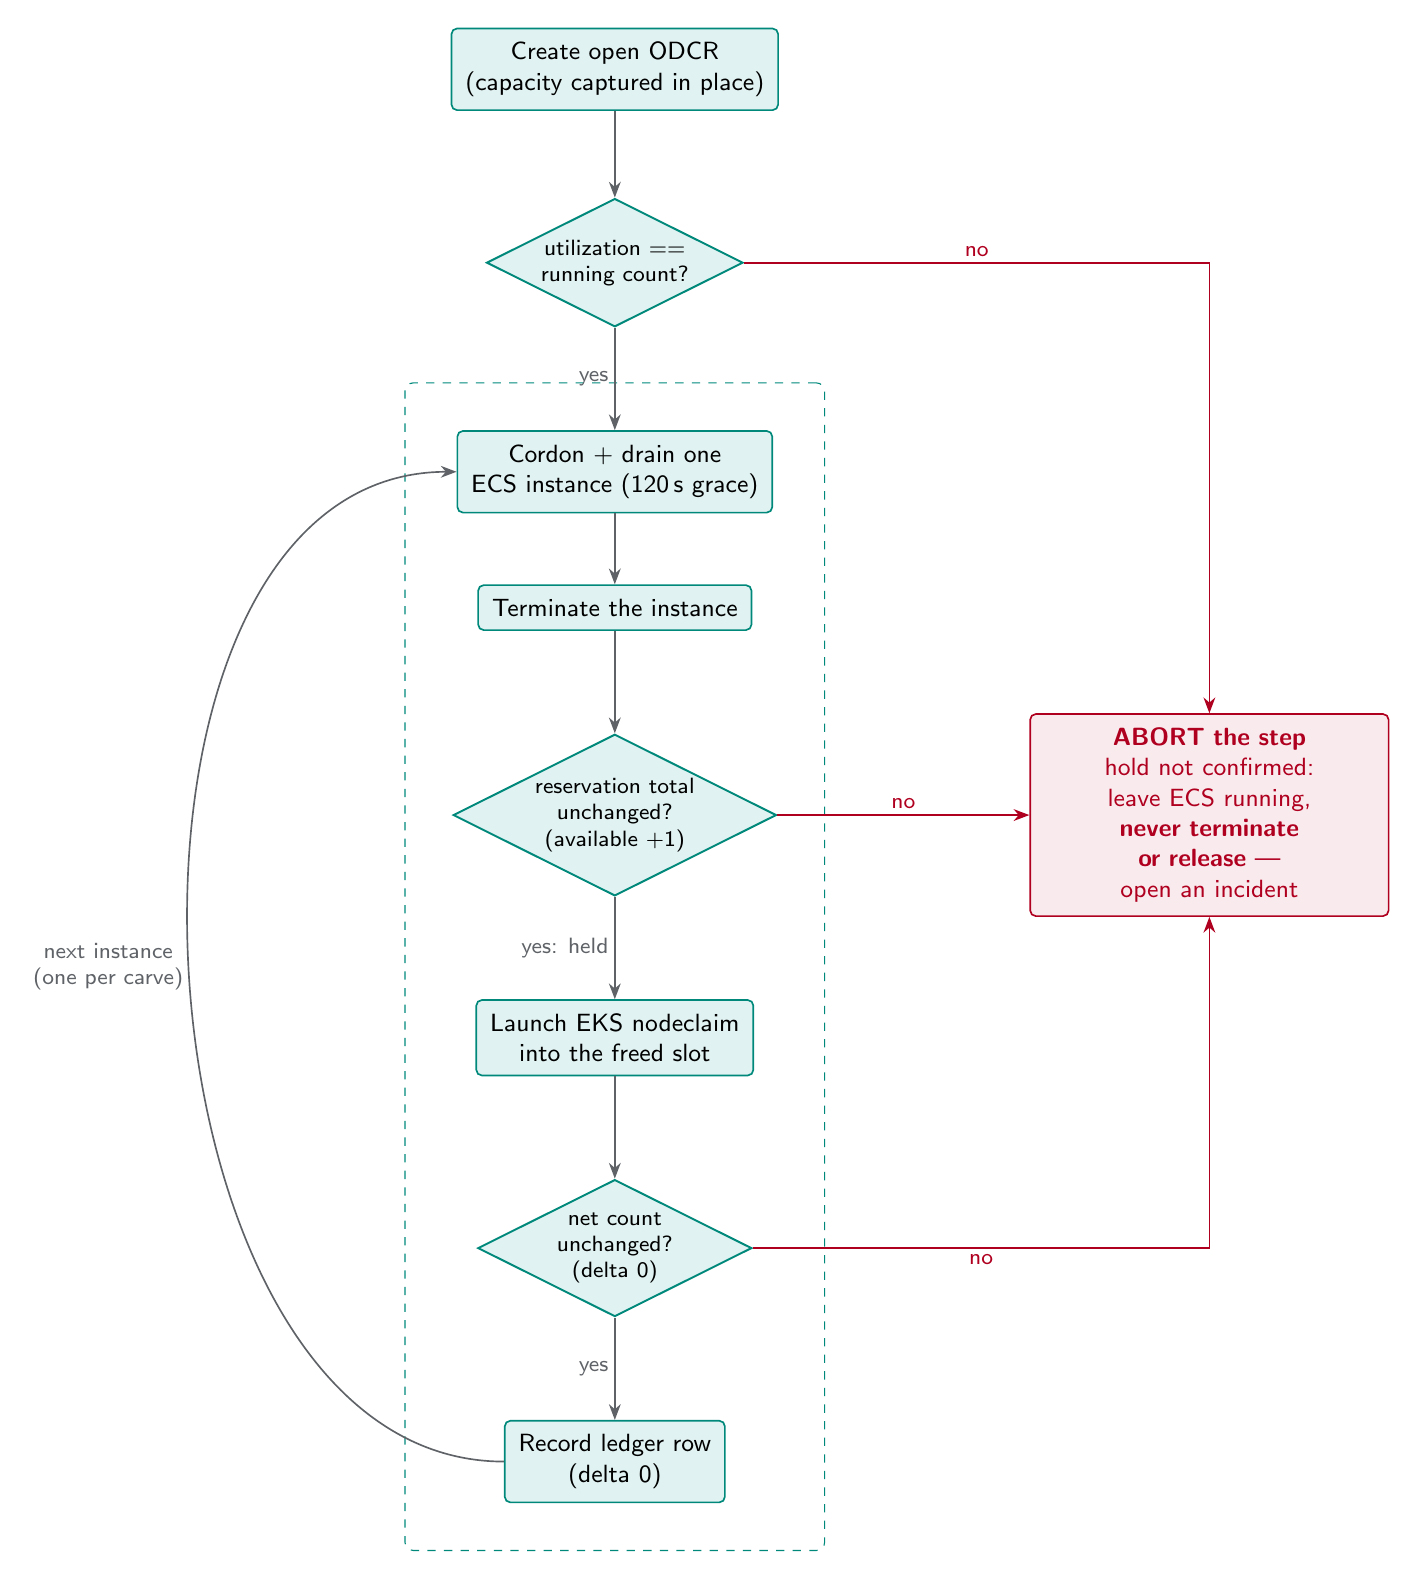
\begin{tikzpicture}[node distance=9mm and 30mm]
  \node[box] (odcr) {Create open ODCR\\(capacity captured in place)};
  \node[decision,below=11mm of odcr] (v0) {utilization ==\\running count?};
  \node[box,below=13mm of v0] (drain) {Cordon + drain one\\ECS instance (120\,s grace)};
  \node[box,below=of drain] (term) {Terminate the instance};
  \node[decision,below=13mm of term] (v1) {reservation total\\unchanged?\\(available +1)};
  \node[box,below=13mm of v1] (launch) {Launch EKS nodeclaim\\into the freed slot};
  \node[decision,below=13mm of launch] (v2) {net count\\unchanged?\\(delta 0)};
  \node[box,below=13mm of v2] (ledger) {Record ledger row\\(delta 0)};

  % one shared ABORT terminal — the never-release invariant, made obvious
  \node[box,deny,right=32mm of v1,text width=42mm] (abort)
    {\textbf{ABORT the step}\\hold not confirmed:\\leave ECS running,\\\textbf{never terminate\\or release} ---\\open an incident};

  \draw[flow] (odcr) -- (v0);
  \draw[flow] (v0) -- node[flowlbl,left]{yes} (drain);
  \draw[flow] (drain) -- (term);
  \draw[flow] (term) -- (v1);
  \draw[flow] (v1) -- node[flowlbl,left]{yes: held} (launch);
  \draw[flow] (launch) -- (v2);
  \draw[flow] (v2) -- node[flowlbl,left]{yes} (ledger);

  % every failed hold routes to the same ABORT (fail closed on capacity)
  \draw[flow,draw=synred] (v0.east) -| node[flowlbl,text=synred,near start,above]{no} (abort.north);
  \draw[flow,draw=synred] (v1.east) -- node[flowlbl,text=synred,above]{no} (abort.west);
  \draw[flow,draw=synred] (v2.east) -| node[flowlbl,text=synred,near start,below]{no} (abort.south);

  % loop to the next carve — one instance per invocation
  \draw[flow] (ledger.west) to[out=180,in=180]
    node[flowlbl,left,align=center]{next instance\\(one per carve)} (drain.west);

  \begin{scope}[on background layer]
    \node[draw=synteal,dashed,rounded corners=3pt,inner sep=6mm,
          fit=(drain)(v1)(launch)(v2)(ledger)] {};
  \end{scope}
\end{tikzpicture}
\end{document}
